% ju 26-Nov-24 Python-Umgebung.tex
\documentclass{vorlage-design-main}

% Checkbox Definition
\newcommand{\checkbox}{\square}


%% Ganze Überschrift
\title{}
%% Kürzerer Titel zur Verwendung im Seitenkopf
\runningtitle{}
\author{Jan Unger}
\date{\today}

%% Die .bib-Datei mit vollständigen Referenzen zur Verwendung mit biblatex. 
%% articleclass lädt das Paket biblatex-chicago mit Anpassungen
\addbibresource{literatur.bib}

\begin{document}

\maketitle

\begin{abstract}



\end{abstract}

\section{Python - Verwendung von virtuellen
Umgebungen}\label{python---verwendung-von-virtuellen-umgebungen}

\begin{enumerate}
\def\labelenumi{\arabic{enumi}.}
\item
  Deaktivieren Sie zuerst Ihre aktuelle virtuelle Umgebung:

\begin{lstlisting}
deactivate
\end{lstlisting}
\item
  Erstellen Sie eine neue virtuelle Umgebung:

\begin{lstlisting}
python3 -m venv myenv_new
\end{lstlisting}
\item
  Aktivieren Sie die neue Umgebung:

\begin{lstlisting}
source myenv_new/bin/activate
\end{lstlisting}
\item
  Überprüfen Sie, ob Sie jetzt die richtige Python-Version verwenden:

\begin{lstlisting}
which python3
\end{lstlisting}

  Dies sollte nun einen Pfad in Ihrer neuen virtuellen Umgebung
  anzeigen, etwa
  \verb|/path/to/myenv\_new/bin/python3|.
\item
  Wenn der Pfad korrekt ist, versuchen Sie erneut, PyYAML zu
  installieren:

\begin{lstlisting}
python3 -m pip install PyYAML
\end{lstlisting}
\item
  Wenn die Installation erfolgreich war, können Sie Ihr Skript in dieser
  neuen Umgebung ausführen:

\begin{lstlisting}
python3 ./scriptauswahl.py
\end{lstlisting}
\item
  Um die Ausgabe mit einem benutzerdefinierten Header zu versehen:

\begin{lstlisting}
(
echo "Installed Python packages in myenv_system environment:"
echo "Date: $(date)"
echo "----------------------------------------"
pip list --format=freeze | cut -d '=' -f 1
) > installed_packages.txt
\end{lstlisting}
\item
  Inhalt im Terminal anzeigen:
\end{enumerate}

\begin{lstlisting}
cat installed_packages.txt
\end{lstlisting}

\subsection{Keywords: Datenwissenschaft und Maschinelles Lernen mit
Python}\label{keywords-datenwissenschaft-und-maschinelles-lernen-mit-python}

\begin{itemize}

\item
  Keywords: Python, maschinelles Lernen, Pandas, NumPy, SciPy,
  Matplotlib, Seaborn, Plotly, Traditionelles Maschinelles Lernen,
  Scikit-learn, Supervised Learning, Unsupervised Learning, Tiefes
  Lernen, TensorFlow, Training tiefer neuronaler Netzwerke,
  Bilderkennung, PyTorch, Jupyter Notebooks, Explorative Datenanalyse,
  Statistische Grafiken, Verständnis von Datenmustern, Algorithmen,
  Regression, Klassifikation, Überwachtes Lernen
\end{itemize}

\subsubsection{Python}\label{python}

Python ist eine vielseitige Programmiersprache, ähnlich einem Schweizer
Taschenmesser für Entwickler und Wissenschaftler. Sie ermöglicht die
Lösung einfacher Aufgaben wie das Sortieren einer Liste von Namen ebenso
effizient wie die Durchführung komplexer Datenanalysen oder das
Entwickeln von Lernalgorithmen für künstliche Intelligenz.

\subsubsection{Maschinelles Lernen}\label{maschinelles-lernen}

Maschinelles Lernen ist vergleichbar mit dem Lernprozess eines Kindes,
das aus Erfahrungen lernt. Statt zu sagen: >>Das ist ein Hund<<, lernt
der Computer aus vielen Bildern, was einen Hund kennzeichnet, und kann
schließlich selbstständig Hunde auf Bildern erkennen.

\subsubsection{Pandas}\label{pandas}

Pandas ist eine Bibliothek in Python, die als multifunktionales Werkzeug
für Datenanalysten und Wissenschaftler dient. Sie kann als ein extrem
effizientes und flexibles Werkzeug betrachtet werden, das Daten
sortieren, bereinigen und analysieren kann, ähnlich einem
Taschenrechner, der speziell für die Arbeit mit großen Datensätzen
konzipiert wurde.

\subsubsection{NumPy}\label{numpy}

NumPy erweitert die Fähigkeiten von Python, indem es Unterstützung für
große, mehrdimensionale Arrays und Matrizen bietet, zusammen mit einer
umfangreichen Sammlung von mathematischen Funktionen. Man kann es als
das Fundament eines Gebäudes betrachten, auf dem komplexere
Datenanalyse- und Wissenschaftsprojekte aufgebaut sind.

\subsubsection{SciPy}\label{scipy}

SciPy nutzt NumPy, um weitere Funktionalitäten für wissenschaftliches
Rechnen hinzuzufügen, wie Optimierung, Statistik und Signalverarbeitung.
Es ist wie ein erweitertes Laborwerkzeug, das spezielle Instrumente für
verschiedene wissenschaftliche Aufgaben bereitstellt.

\subsubsection{Matplotlib, Seaborn,
Plotly}\label{matplotlib-seaborn-plotly}

Diese Bibliotheken dienen der Datenvisualisierung. Matplotlib ermöglicht
grundlegende Grafiken und Diagramme, Seaborn fügt attraktive Designs und
einfache Schnittstellen für komplexe statistische Grafiken hinzu, und
Plotly erlaubt interaktive, webbasierte Grafiken. Zusammen bilden sie
ein Toolkit, vergleichbar mit einem Satz von Zeichenwerkzeugen, der es
ermöglicht, Daten in visuell ansprechender Form darzustellen.

\subsubsection{Traditionelles Maschinelles Lernen und
Scikit-learn}\label{traditionelles-maschinelles-lernen-und-scikit-learn}

Traditionelles maschinelles Lernen mit Scikit-learn beinhaltet Techniken
wie Regression und Klassifikation. Man kann sich das vorstellen wie das
Erlernen der Grundlagen des Autofahrens: Bevor man lernt, wie man ein
Rennauto fährt (tiefe neuronale Netzwerke), muss man mit einem normalen
Auto umgehen können, einschließlich des Schaltens, Lenkens und Parkens.

\subsubsection{Supervised und Unsupervised
Learning}\label{supervised-und-unsupervised-learning}

Supervised Learning ist, als würde man einem Kind beibringen, Rad zu
fahren, indem man es an der Hand hält und ihm Richtungen gibt.
Unsupervised Learning hingegen ist wie das Erkunden eines unbekannten
Raumes ohne Anleitung, um selbst Muster oder Strukturen zu erkennen.

\subsubsection{Tiefes Lernen, TensorFlow und
PyTorch}\label{tiefes-lernen-tensorflow-und-pytorch}

Tiefes Lernen mit TensorFlow oder PyTorch ist vergleichbar mit dem Bau
und der Feinabstimmung eines Raumschiffs. Es handelt sich um
fortschrittliche Werkzeuge, die es ermöglichen, komplexe Modelle zu
entwickeln, die Aufgaben wie Bild- und Spracherkennung durchführen
können, weit über das hinaus, was mit traditionellem maschinellem Lernen
möglich ist.

\subsubsection{Jupyter Notebooks}\label{jupyter-notebooks}

Jupyter Notebooks sind interaktive Dokumente, die Code, Text und
Visualisierungen kombinieren. Sie sind vergleichbar mit einem
Laborjournal, in dem Wissenschaftler ihre Experimente dokumentieren,
durchführen und die Ergebnisse für andere sichtbar machen können.

\subsubsection{Explorative Datenanalyse und Statistische
Grafiken}\label{explorative-datenanalyse-und-statistische-grafiken}

Explorative Datenanalyse ist der Prozess des Durchstöberns von Daten, um
Einsichten und Muster zu finden, ähnlich einem Detektiv, der nach
Hinweisen sucht. Statistische Grafiken helfen dabei, diese Muster
sichtbar zu machen, wie eine Lupe, die kleinste Details hervorhebt.

\subsubsection{Algorithmen, Regression, Klassifikation und Überwachtes
Lernen}\label{algorithmen-regression-klassifikation-und-ueberwachtes-lernen}

Algorithmen sind die Rezepte des maschinellen Lernens,
Schritt-für-Schritt-Anweisungen, um Daten zu analysieren und Vorhersagen
zu treffen. Regression und Klassifikation sind zwei grundlegende Arten
des überwachten Lernens, vergleichbar mit dem Lösen von Gleichungen in
der Mathematik bzw. dem Ordnen von Objekten in Kategorien in der
Biologie.

\newpage

\subsection{Mindmap: Datenwissenschaft und Maschinelles Lernen mit
Python}\label{mindmap-datenwissenschaft-und-maschinelles-lernen-mit-python}

\textbf{Zentrales Thema: Datenwissenschaft und Maschinelles Lernen mit
Python.}

\begin{enumerate}
\def\labelenumi{\arabic{enumi}.}

\item
  Grundlegende Bibliotheken

  \begin{itemize}
  
  \item
    \textbf{Pandas}

    \begin{itemize}
    
    \item
      Datenmanipulation
    \item
      Datenreinigung
    \item
      Zeitreihenanalyse
    \end{itemize}
  \item
    \textbf{NumPy}

    \begin{itemize}
    
    \item
      Mehrdimensionale Arrays
    \item
      Mathematische Operationen
    \end{itemize}
  \item
    \textbf{SciPy}

    \begin{itemize}
    
    \item
      Wissenschaftliches Rechnen
    \item
      Statistik
    \item
      Optimierungsaufgaben
    \end{itemize}
  \end{itemize}
\item
  Datenvisualisierung

  \begin{itemize}
  
  \item
    \textbf{Matplotlib}

    \begin{itemize}
    
    \item
      Basisdiagramme und -grafiken
    \item
      Anpassung von Plots
    \end{itemize}
  \item
    \textbf{Seaborn}

    \begin{itemize}
    
    \item
      Statistische Grafiken
    \item
      Attraktive Standarddesigns
    \end{itemize}
  \item
    \textbf{Plotly}

    \begin{itemize}
    
    \item
      Interaktive, webbasierte Grafiken
    \item
      Komplexere Visualisierungen
    \end{itemize}
  \end{itemize}
\item
  Maschinelles Lernen

  \begin{itemize}
  
  \item
    \textbf{Traditionelles Maschinelles Lernen}

    \begin{itemize}
    
    \item
      \textbf{Scikit-learn}

      \begin{itemize}
      
      \item
        Algorithmen für Supervised Learning (z.B. Regression,
        Klassifikation)
      \item
        Algorithmen für Unsupervised Learning (z.B. Clustering)
      \end{itemize}
    \end{itemize}
  \item
    \textbf{Tiefes Lernen}

    \begin{itemize}
    
    \item
      \textbf{TensorFlow}

      \begin{itemize}
      
      \item
        Aufbau und Training tiefer neuronaler Netzwerke
      \item
        Anwendungsbereiche (Bilderkennung, Sprachverarbeitung)
      \end{itemize}
    \item
      \textbf{PyTorch}

      \begin{itemize}
      
      \item
        Dynamische Berechnungsgraphen
      \item
        Forschungsfreundlich
      \end{itemize}
    \end{itemize}
  \end{itemize}
\item
  Entwicklungsumgebung

  \begin{itemize}
  
  \item
    \textbf{Jupyter Notebooks}

    \begin{itemize}
    
    \item
      Interaktive Code-Ausführung
    \item
      Integration von Text, Code und Visualisierungen
    \end{itemize}
  \end{itemize}
\item
  Schlüsselkonzepte

  \begin{itemize}
  
  \item
    \textbf{Datenanalyse}

    \begin{itemize}
    
    \item
      Explorative Datenanalyse
    \item
      Datenbereinigung und -vorbereitung
    \end{itemize}
  \item
    \textbf{Statistische Grafiken}

    \begin{itemize}
    
    \item
      Verständnis von Datenmustern
    \end{itemize}
  \item
    \textbf{Explorative Datenanalyse}

    \begin{itemize}
    
    \item
      Erste Schritte der Datenuntersuchung
    \end{itemize}
  \item
    \textbf{Algorithmen}

    \begin{itemize}
    
    \item
      Verstehen, wie maschinelles Lernen funktioniert
    \end{itemize}
  \item
    \textbf{Regression und Klassifikation}

    \begin{itemize}
    
    \item
      Zwei Haupttypen des überwachten Lernens
    \end{itemize}
  \end{itemize}
\end{enumerate}

\subsection{Mindmap: Python, Anaconda und Jupyter Notebooks in der
Datenwissenschaft}\label{mindmap-python-anaconda-und-jupyter-notebooks-in-der-datenwissenschaft}

\begin{figure}
\centering
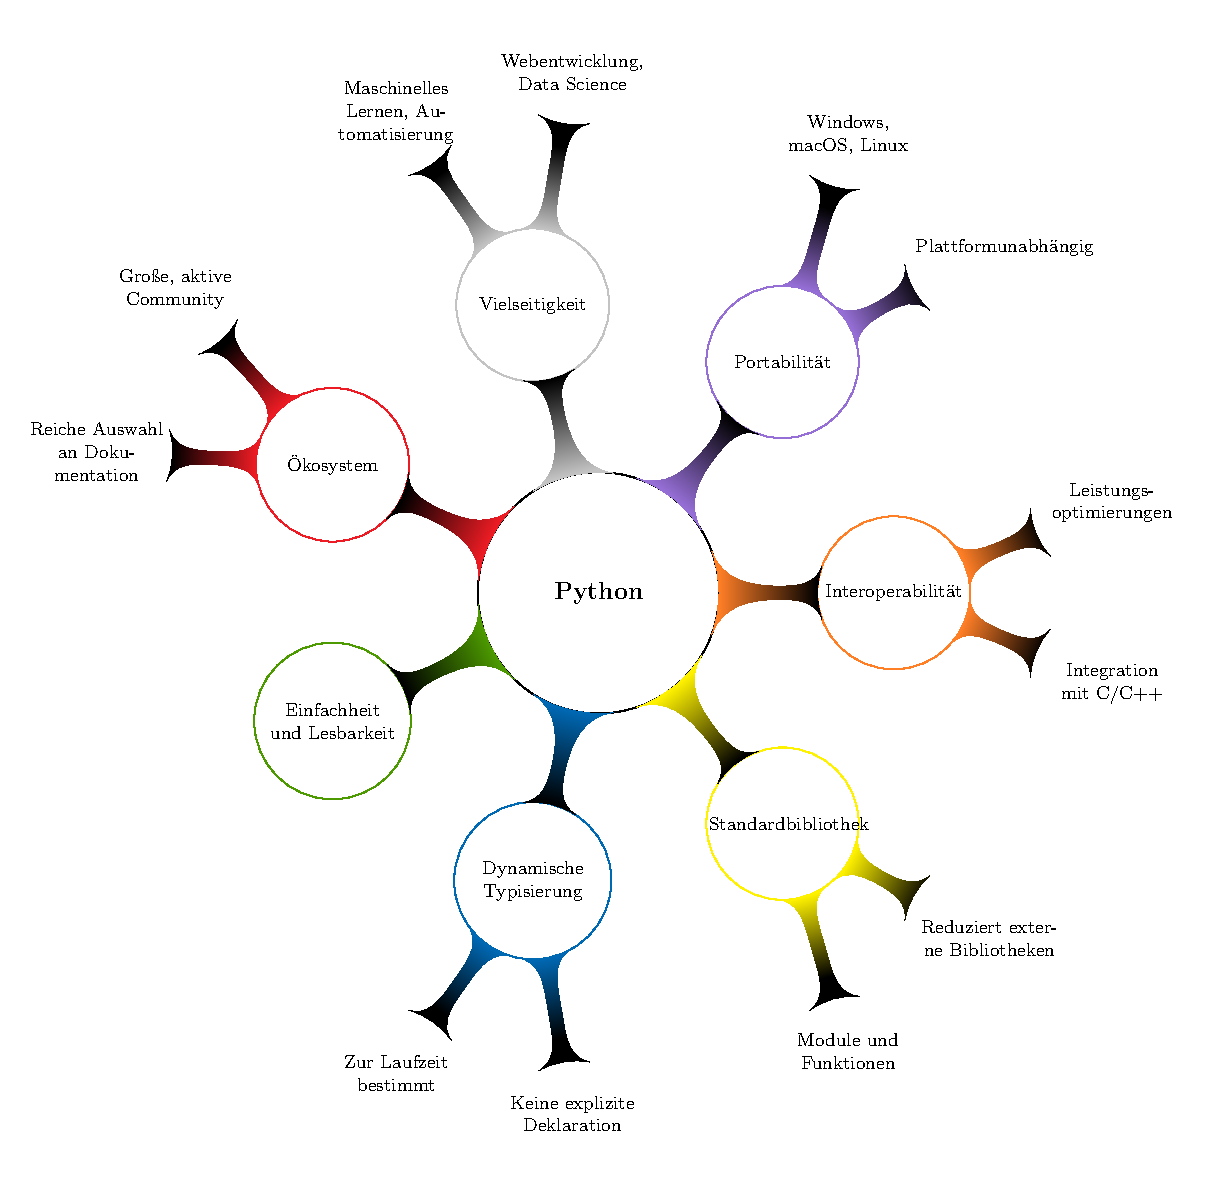
\includegraphics[keepaspectratio]{images/Mindmap-Python.pdf}
\caption{PDF: Mindmap - Python}
\end{figure}

\textbf{Zentrales Thema: Python, Anaconda und Jupyter Notebooks in der
Datenwissenschaft.}

\begin{enumerate}
\def\labelenumi{\arabic{enumi}.}

\item
  \textbf{Python}

  \begin{itemize}
  
  \item
    Definition: Hochrangige Programmiersprache
  \item
    Eigenschaften

    \begin{itemize}
    
    \item
      Klarheit
    \item
      Einfachheit
    \end{itemize}
  \item
    Anwendungsbereiche

    \begin{itemize}
    
    \item
      Programmierung
    \item
      Datenanalyse
    \end{itemize}
  \item
    Unterstützung durch Bibliotheken
  \end{itemize}
\item
  \textbf{Anaconda}

  \begin{itemize}
  
  \item
    Definition: Open-Source-Distribution für Python und R
  \item
    Rolle: Werkzeugkasten für Datenwissenschaftler
  \item
    Hauptmerkmale

    \begin{itemize}
    
    \item
      Vereinfachung von Installation und Verwaltung
    \item
      Sammlung von Bibliotheken für Datenwissenschaft und maschinelles
      Lernen
    \end{itemize}
  \end{itemize}
\item
  \textbf{Jupyter Notebooks}

  \begin{itemize}
  
  \item
    Definition: Open-Source-Webanwendung
  \item
    Funktionen

    \begin{itemize}
    
    \item
      Erstellung lebendiger Dokumente
    \item
      Integration von Code, Gleichungen und Visualisierungen
    \end{itemize}
  \item
    Nutzungskontext

    \begin{itemize}
    
    \item
      Explorative Datenanalyse
    \item
      Bildung
    \item
      Projektzusammenarbeit
    \end{itemize}
  \end{itemize}
\item
  \textbf{Synergie und Integration}

  \begin{itemize}
  
  \item
    Verbindung der Komponenten

    \begin{itemize}
    
    \item
      Python als Basis
    \item
      Anaconda als vereinfachende Plattform
    \item
      Jupyter Notebooks als interaktive Arbeitsumgebung
    \end{itemize}
  \item
    Anwendungsszenarien

    \begin{itemize}
    
    \item
      Datenaufbereitung
    \item
      Analyse
    \item
      Visualisierung
    \item
      Präsentation
    \end{itemize}
  \end{itemize}
\item
  \textbf{Praktische Anwendung}

  \begin{itemize}
  
  \item
    Effizienz in der Datenwissenschaft

    \begin{itemize}
    
    \item
      Schneller Einstieg durch Anaconda
    \item
      Flexibilität und Leistungsfähigkeit durch Python
    \item
      Interaktivität und Dokumentation durch Jupyter Notebooks
    \end{itemize}
  \item
    Kooperation und Kommunikation

    \begin{itemize}
    
    \item
      Gemeinsame Nutzung von Notebooks
    \item
      Erleichterung der Zusammenarbeit und des Lernens
    \end{itemize}
  \end{itemize}
\end{enumerate}

\newpage

\subsection{Kewords: Python, Anaconda, Jupyter
Notebooks}\label{kewords-python-anaconda-jupyter-notebooks}

\begin{itemize}

\item
  \textbf{Kewords}: Python, Anaconda, Jupyter Notebooks, Programmierung,
  Bibliotheken, Datenwissenschaft, maschinelles Lernen, explorative
  Datenanalyse, Pandas, Scikit-learn, Matplotlib, Seaborn
\end{itemize}

\subsubsection{Was ist Python?}\label{was-ist-python}

Python ist eine Programmiersprache, ähnlich wie Englisch eine Sprache
für die Kommunikation zwischen Menschen ist. Python wird wegen seiner
Klarheit und Einfachheit geschätzt, ähnlich wie ein einfaches Werkzeug,
das für viele Aufgaben verwendet werden kann. In der Datenwissenschaft
ermöglicht Python es, mit Daten zu >>sprechen<<, sie zu analysieren und
aus ihnen zu lernen.

\subsubsection{Was ist Anaconda?}\label{was-ist-anaconda}

Anaconda kann man sich als einen großen Koffer für einen Wissenschaftler
vorstellen, der alle Instrumente und Geräte enthält, die für Experimente
benötigt werden. In diesem Koffer finden sich alle möglichen Werkzeuge
(Bibliotheken und Programme) für die Datenwissenschaft und das
maschinelle Lernen, vorinstalliert und bereit zur Verwendung mit Python.
Anaconda vereinfacht die Organisation und den Zugriff auf diese
Werkzeuge erheblich.

\subsubsection{Was ist Jupyter
Notebooks?}\label{was-ist-jupyter-notebooks}

Jupyter Notebooks sind wie interaktive Notizbücher, in denen
Wissenschaftler ihre Gedanken (Code und Anmerkungen) sowie die
Ergebnisse ihrer Experimente (Grafiken und Daten) festhalten können.
Diese digitalen Notizbücher unterstützen die explorative Datenanalyse,
indem sie die unmittelbare Ausführung von Code und die Visualisierung
der Ergebnisse in einem einzigen Dokument ermöglichen.

\subsubsection{Programmierung}\label{programmierung}

Programmierung in diesem Kontext bezieht sich auf den Prozess der
Erstellung von Instruktionen, die es dem Computer ermöglichen, mit Daten
umzugehen und aus ihnen zu lernen. Es ist vergleichbar mit dem Schreiben
eines Rezeptes, das genau beschreibt, welche Zutaten benötigt werden und
wie sie zu einem Gericht verarbeitet werden.

\subsubsection{Bibliotheken}\label{bibliotheken}

Bibliotheken in Python sind Sammlungen von Werkzeugen und Funktionen,
die spezifische Aufgaben erleichtern. Man kann sie sich vorstellen wie
Bücher in einer Bibliothek, die Wissen zu bestimmten Themen
bereitstellen. Statt jedes Mal ein Buch von Grund auf neu zu schreiben,
nutzen Wissenschaftler diese Bücher, um schnell auf bestehendes Wissen
zuzugreifen.

\subsubsection{Datenwissenschaft}\label{datenwissenschaft}

Datenwissenschaft ist das Feld, das Methoden und Techniken nutzt, um aus
großen Mengen von Daten nützliche Informationen zu gewinnen. Man kann es
mit der Archäologie vergleichen, bei der aus verstreuten Fragmenten
wertvolle Artefakte und Wissen über vergangene Zivilisationen
zusammengetragen werden.

\subsubsection{Was ist Maschinelles
Lernen?}\label{was-ist-maschinelles-lernen}

Maschinelles Lernen ist ein Bereich innerhalb der Datenwissenschaft, der
Computern die Fähigkeit gibt, aus Daten zu lernen, ohne explizit
programmiert zu sein. Es ist, als würde man einem Roboter beibringen,
aus Erfahrungen zu lernen und seine Aufgaben mit der Zeit besser zu
erfüllen.

\subsubsection{Was ist Explorative
Datenanalyse?}\label{was-ist-explorative-datenanalyse}

Explorative Datenanalyse ist der Prozess des ersten >>Erkundens<< der
Daten, um Muster, Anomalien oder interessante Beziehungen zu entdecken,
ohne vorher spezifische Hypothesen zu haben. Es ist wie das erste Öffnen
einer Schatzkiste, um zu sehen, was darin versteckt ist.

\subsubsection{Was ist Pandas?}\label{was-ist-pandas}

Pandas ist eine Bibliothek in Python, speziell entwickelt für die
Datenmanipulation und -analyse. Man kann sich Pandas als ein
multifunktionales Schweizer Taschenmesser vorstellen, das für die Arbeit
mit tabellarischen Daten optimiert ist.

\subsubsection{Scikit-learn}\label{scikit-learn}

Scikit-learn ist eine Bibliothek für maschinelles Lernen in Python. Sie
bietet einfache und effiziente Werkzeuge für Datenmining und
Datenanalyse. Man kann sich Scikit-learn als einen Werkzeugkasten
vorstellen, der alle notwendigen Werkzeuge für den Bau und das
Verständnis komplexer maschineller Lernmodelle enthält.

\subsubsection{Matplotlib und Seaborn}\label{matplotlib-und-seaborn}

Matplotlib und Seaborn sind Bibliotheken für die Datenvisualisierung in
Python. Während Matplotlib grundlegende Grafiken und Diagramme
ermöglicht, baut Seaborn darauf auf und bietet eine höhere
Abstraktionsebene für die Erstellung statistisch anspruchsvoller
Visualisierungen. Zusammen bieten sie das künstlerische Werkzeug, mit
dem Wissenschaftler die Geschichte ihrer Daten durch visuelle
Darstellungen erzählen können.

\subsection{Homebrew (kurz >>brew<<), dem Paketmanager für
macOS}\label{homebrew-kurz-brew-dem-paketmanager-fuer-macos}

\begin{lstlisting}[language=bash]
# Homebrew installieren
/bin/bash -c "$(curl -fsSL https://raw.githubusercontent.com/Homebrew/install/HEAD/install.sh)"

# Homebrew aktualisieren
brew update
brew upgrade
brew cleanup
brew doctor

brew install <paketname>
# Installierte Pakete auflisten
brew list
# Informationen über ein Paket anzeigen
brew info <paketname>
# Paket aktualisieren
brew upgrade <paketname>
brew uninstall <paketname>
# Suche nach Paketen
brew search <suchbegriff>
# Abhängigkeiten anzeigen
brew deps <paketname>

# php, mysql, apache, mosquitto (ESP32)
brew services list
brew services restart httpd
brew services restart mosquitto
brew services restart mysql
brew services restart php

# Systeminfo
brew install neofetch
neofetch
\end{lstlisting}

\subsection{Namenskonventionen für HostName, LocalHostName und
ComputerName}\label{namenskonventionen-fuer-hostname-localhostname-und-computername}

\begin{enumerate}
\def\labelenumi{\arabic{enumi}.}

\item
  \textbf{HostName:}

  \begin{itemize}
  \item
    \textbf{Ziel:} Ein eindeutiger, vollqualifizierter Domänenname
    (FQDN) für die Netzwerkdienste und Unix-Befehle.
  \item
    \textbf{Empfehlung:} imacj.example.com
  \item
    \textbf{Befehl:}

\begin{lstlisting}[language=bash]
sudo scutil --set HostName imacj.example.com
\end{lstlisting}
  \end{itemize}
\item
  \textbf{LocalHostName:}

  \begin{itemize}
  \item
    \textbf{Ziel:} Ein eindeutiger Name für die lokale
    Netzwerkerkennung, der von Bonjour verwendet wird. Dieser Name
    sollte keine Leerzeichen oder Sonderzeichen enthalten und in
    Kleinbuchstaben sein.
  \item
    \textbf{Empfehlung:} imacj
  \item
    \textbf{Befehl:}

\begin{lstlisting}[language=bash]
sudo scutil --set LocalHostName imacj
\end{lstlisting}
  \end{itemize}
\item
  \textbf{ComputerName:}

  \begin{itemize}
  \item
    \textbf{Ziel:} Ein benutzerfreundlicher Name, der in der
    macOS-Oberfläche und Netzwerkerkennung angezeigt wird.
  \item
    \textbf{Empfehlung:} iMac von Jan
  \item
    \textbf{Befehl:}

\begin{lstlisting}[language=bash]
sudo scutil --set ComputerName "iMac von Jan"
\end{lstlisting}
  \end{itemize}
\end{enumerate}

\subsubsection{Schritte zur Umsetzung:}\label{schritte-zur-umsetzung}

\begin{enumerate}
\def\labelenumi{\arabic{enumi}.}
\item
  \textbf{Setze den HostName:}

\begin{lstlisting}[language=bash]
sudo scutil --set HostName imacj.example.com
\end{lstlisting}
\item
  \textbf{Setze den LocalHostName:}

\begin{lstlisting}[language=bash]
sudo scutil --set LocalHostName imacj
\end{lstlisting}
\item
  \textbf{Setze den ComputerName:}

\begin{lstlisting}[language=bash]
sudo scutil --set ComputerName "iMac von Jan"
\end{lstlisting}
\item
  \textbf{Überprüfe die Änderungen:}

\begin{lstlisting}[language=bash]
scutil --get HostName
scutil --get LocalHostName
scutil --get ComputerName
\end{lstlisting}
\end{enumerate}

\subsubsection{Erklärung}\label{erklaerung}

\begin{itemize}

\item
  \textbf{HostName (imacj.example.com):} Der HostName wird verwendet,
  wenn der Mac in größeren Netzwerken oder durch Dienste und Skripte
  eindeutig identifiziert werden muss. Die Verwendung eines
  vollqualifizierten Domänennamens (FQDN) sorgt für Eindeutigkeit.
\item
  \textbf{LocalHostName (imacj):} Der LocalHostName wird von Bonjour für
  die lokale Netzwerkerkennung verwendet. Ein kurzer, prägnanter Name
  ohne Sonderzeichen oder Leerzeichen erleichtert die Identifikation.
\item
  \textbf{ComputerName (iMac von Jan):} Der ComputerName ist der
  benutzerfreundliche Name, der in der macOS-Benutzeroberfläche
  angezeigt wird. Die Verwendung eines verständlichen Namens macht es
  einfacher, den Mac in Netzwerken oder in der Systemeinstellung
  >>Freigaben<< zu identifizieren.
\end{itemize}

Durch diese Namenskonventionen wird sichergestellt, dass dein Mac sowohl
technisch einwandfrei als auch benutzerfreundlich und eindeutig im
Netzwerk identifiziert wird.

\subsection{zshrc}\label{zshrc}

\begin{lstlisting}[language=bash]
vim ~/.zshrc
source ~/.zshrc

# ~/.zshrc
# Hilfsfunktion, um Verzeichnisse zum $PATH hinzuzufügen, wenn sie noch nicht vorhanden sind
add_to_path() {
    for dir in "$@"; do
        if [[ -d "$dir" && ":$PATH:" != *":$dir:"* ]]; then
            PATH="$dir:$PATH"
        fi
    done
}

# Systemweite Python-Installation zuerst setzen
export PATH="/usr/local/bin:/usr/bin:/bin:/usr/sbin:/sbin"

# Ruby-Initialisierung (falls vorhanden)
if command -v rbenv > /dev/null; then
  eval "$(rbenv init -)"
fi

# Node Version Manager (NVM) Initialisierung
export NVM_DIR="$HOME/.nvm"
[ -s "$NVM_DIR/nvm.sh" ] && \. "$NVM_DIR/nvm.sh"
[ -s "$NVM_DIR/bash_completion" ] && \. "$NVM_DIR/bash_completion"

# LLVM-Umgebungsvariablen
export LDFLAGS="-L/usr/local/opt/llvm/lib"
export CPPFLAGS="-I/usr/local/opt/llvm/include"

# Weitere Pfade hinzufügen
add_to_path \
    "$HOME/bin" \
    "$HOME/Downloads/flutter/bin" \
    "$HOME/.local/bin" \
    "$HOME/esp/esp-idf" \
    /usr/local/opt/llvm/bin \
    /usr/local/opt/openjdk/bin \
    /Library/TeX/texbin \
    /Library/Apple/usr/bin \
    /System/Cryptexes/App/usr/bin \
    /var/run/com.apple.security.cryptexd/codex.system/bootstrap/usr/local/bin \
    /var/run/com.apple.security.cryptexd/codex.system/bootstrap/usr/bin \
    /var/run/com.apple.security.cryptexd/codex.system/bootstrap/usr/appleinternal/bin

# Aliase
alias ll="ls -laG"
alias ls='ls -G'
alias python=python3
alias maintenancetool='/Users/jan/Qt/MaintenanceTool.app/Contents/MacOS/MaintenanceTool'

# Funktion zum Laden von pyenv
load_pyenv() {
    export PATH="$HOME/.pyenv/bin:$PATH"
    eval "$(pyenv init --path)"
    eval "$(pyenv init -)"
    eval "$(pyenv virtualenv-init -)"
}

# Funktion zum Laden von Anaconda
load_anaconda() {
    if [[ -d "$HOME/anaconda3" ]]; then
        export CONDA_PREFIX="$HOME/anaconda3"
        __conda_setup="$("$CONDA_PREFIX/bin/conda" 'shell.zsh' 'hook' 2> /dev/null)"
        if [ $? -eq 0 ]; then
            eval "$__conda_setup"
        else
            if [ -f "$CONDA_PREFIX/etc/profile.d/conda.sh" ]; then
                . "$CONDA_PREFIX/etc/profile.d/conda.sh"
            fi
        fi
        unset __conda_setup
        export PATH="$CONDA_PREFIX/bin:$PATH"
    fi
}

# Prompt-Einstellungen
unsetopt PROMPT_SUBST

# Farben definieren
autoload -U colors && colors

# Git-Branch anzeigen, falls im Git-Repository
parse_git_branch() {
  git branch 2>/dev/null | sed -n '/\* /s///p'
}

# Prompt definieren
PROMPT='%{$fg[green]%}%n@%m%{$reset_color%}:%{$fg[blue]%}%~%{$reset_color%}$(parse_git_branch) $ '

# Wenn in einem Git-Repository, zeige den aktuellen Branch in Rot
RPROMPT='$(parse_git_branch)'

# Optionen, um die Farben des Prompts anzupassen
setopt prompt_subst
\end{lstlisting}

\subsection{Aktualisieren der
Python-Version}\label{aktualisieren-der-python-version}

\subsubsection{Systemweite Python - Installation - Erstellen und
Verwalten von virtuellen
Umgebungen}\label{systemweite-python---installation---erstellen-und-verwalten-von-virtuellen-umgebungen}

\begin{lstlisting}[language=bash]
# Aktualisieren von Homebrew
brew update
brew upgrade

# Aktualisieren der Python-Version
brew upgrade python@3.12

# Verlinken der neuesten Python-Version
brew link --force --overwrite python@3.12

# Überprüfen des Pfades und der Python-Version nach dem Update
# HINWEIS: Terminal neu öffnen oder die .zshrc-Datei erneut laden
source ~/.zshrc
which python3
python3 --version

# Anzeigen aller Umgebungen
find ~ -name "activate" -path "*/bin/activate"

# Erstellen und Aktivieren einer virtuellen Umgebung
python3 -m venv myenv_system
source myenv_system/bin/activate

# Überprüfen der Python-Version und des Pfades
python --version  # sollte Python 3.12.4 anzeigen
which python

# Paket-Installation in der virtuellen Umgebung
pip install --upgrade pip
pip install jupyter pandas numpy matplotlib seaborn plotly scikit-learn scipy pyqt5

# Deaktivieren der virtuellen Umgebung
deactivate

# Löschen der virtuellen Umgebung
rm -rf myenv_system
\end{lstlisting}

\subsubsection{\texorpdfstring{\texttt{pyenv}-Installation - Erstellen
und Verwalten von virtuellen
Umgebungen}{pyenv-Installation - Erstellen und Verwalten von virtuellen Umgebungen}}\label{pyenv-installation---erstellen-und-verwalten-von-virtuellen-umgebungen}

\begin{lstlisting}[language=bash]
# Installation von pyenv (falls noch nicht installiert)
brew install pyenv

# Installation von pyenv-virtualenv (falls noch nicht installiert)
brew install pyenv-virtualenv

# Laden von pyenv
# passe an ~/.zshrc
load_pyenv

# Überprüfen der pyenv-Version
pyenv --version

# Anzeigen aller installierten Python-Versionen
pyenv versions

# Installation der gewünschten Python-Version
pyenv install 3.12.4

# Anzeigen aller pyenv-virtuellen Umgebungen
pyenv virtualenvs

# Erstellen einer neuen virtuellen Umgebung mit der gewünschten Python-Version
pyenv virtualenv 3.12.4 myenv

# Aktivieren der neuen virtuellen Umgebung
pyenv activate myenv

# Überprüfen der Python-Version und des Pfades nach der Aktivierung
python --version  # sollte Python 3.12.4 anzeigen
which python

# Installation und Aktualisierung spezifischer Pakete in der virtuellen Umgebung
python3.12 -m pip install --upgrade pip
pip install jupyter pandas numpy matplotlib seaborn plotly scikit-learn scipy pyqt5

# Optional: Installation von Deep Learning-Paketen
# pip install tensorflow torch

# Deaktivieren der virtuellen Umgebung
pyenv deactivate

# Löschen der virtuellen Umgebung
pyenv uninstall myenv
\end{lstlisting}

\subsubsection{Anaconda - Installation - Erstellen und Verwalten von
virtuellen
Umgebungen}\label{anaconda---installation---erstellen-und-verwalten-von-virtuellen-umgebungen}

\begin{lstlisting}[language=bash]
# Installation von Anaconda (falls noch nicht installiert)
brew install --cask anaconda

# Laden von Anaconda
# passe an ~/.zshrc
load_anaconda

# Überprüfen der Conda-Version
conda --version

# Aktualisieren von Conda selbst
conda update conda

# Anzeigen aller Conda-Umgebungen
conda env list

# Erstellen einer neuen Umgebung mit der gewünschten Python-Version
conda create -n py312_env python=3.12

# Aktivieren der neuen Umgebung
conda activate py312_env

# Aktualisieren aller Pakete in der neuen Umgebung
conda update --all

# Installation und Aktualisierung spezifischer Pakete
conda install jupyter pandas numpy matplotlib seaborn plotly scikit-learn scipy pyqt

# Optional: Installation von Deep Learning-Paketen (empfohlen für Python 3.9)
#conda install tensorflow pytorch

# Überprüfen des Pfades und der Python-Version nach der Installation
which python3
python3 --version

conda deactivate
conda remove -n py312_env --all
\end{lstlisting}

\subsection{Installation von Paketen}\label{installation-von-paketen}

\begin{enumerate}
\def\labelenumi{\arabic{enumi}.}

\item
  \textbf{Datenanalyse und -visualisierung}: pandas, numpy, matplotlib,
  seaborn, plotly
\item
  \textbf{Wissenschaftliches Rechnen und numerische Methoden}: numpy,
  scipy, matplotlib
\item
  \textbf{Maschinelles Lernen}: scikit-learn, numpy, pandas, matplotlib
\item
  \textbf{Deep Learning}: tensorflow, pytorch, numpy, pandas (Python 3.9
  empfohlen)
\item
  \textbf{Entwicklung von grafischen Benutzeroberflächen}: pyqt
\end{enumerate}

\subsubsection{Datenanalyse und
-visualisierung}\label{datenanalyse-und--visualisierung}

\begin{lstlisting}[language=bash]
load_anaconda
conda create -n data_analysis_env python=3.12
conda activate data_analysis_env
conda install pandas numpy matplotlib seaborn plotly
conda deactivate
conda remove -n data_analysis_env --all
\end{lstlisting}

\subsubsection{Wissenschaftliches Rechnen und numerische
Methoden}\label{wissenschaftliches-rechnen-und-numerische-methoden}

\begin{lstlisting}[language=bash]
load_anaconda
conda create -n scientific_computing_env python=3.12
conda activate scientific_computing_env
conda install numpy scipy matplotlib
conda deactivate
conda remove -n scientific_computing_env --all
\end{lstlisting}

\subsubsection{Maschinelles-Lernen}\label{maschinelles-lernen-1}

\begin{lstlisting}[language=bash]
load_anaconda
conda create -n ml_env python=3.12
conda activate ml_env
conda install scikit-learn numpy pandas matplotlib
conda deactivate
conda remove -n ml_env --all
\end{lstlisting}

\subsubsection{Deep Learning}\label{deep-learning}

\begin{lstlisting}[language=bash]
load_anaconda
conda create -n deep_learning_env python=3.9  # Python 3.9 empfohlen
conda activate deep_learning_env
conda install tensorflow pytorch numpy pandas
conda deactivate
conda remove -n deep_learning_env --all
\end{lstlisting}

\subsubsection{Entwicklung von grafischen
Benutzeroberflächen}\label{entwicklung-von-grafischen-benutzeroberflaechen}

\begin{lstlisting}[language=bash]
load_anaconda
conda create -n gui_env python=3.12
conda activate gui_env
conda install pyqt
conda deactivate
conda remove -n gui_env --all
\end{lstlisting}

\subsection{Berechtigungen und Ausführrechte
setzen}\label{berechtigungen-und-ausfuehrrechte-setzen}

\begin{lstlisting}[language=bash]
# Berechtigungen für Dateien setzen
find . -type f -name "*.md" -exec chmod 644 {} \;
find . -type f -name "*.txt" -exec chmod 644 {} \;
find . -type f -name "*.html" -exec chmod 644 {} \;
find . -type f -name "*.css" -exec chmod 644 {} \;
find . -type f -name "*.tex" -exec chmod 644 {} \;
find . -type f -name "*.pdf" -exec chmod 644 {} \;

# Ausführrechte für .sh und .py-Dateien setzen
find . -type f -name "*.sh" -exec chmod +x {} \;
find . -type f -name "*.py" -exec chmod +x {} \;

# Berechtigungen für Verzeichnisse setzen
find . -type d -exec chmod 755 {} \;
\end{lstlisting}

\subsection{Anaconda}\label{anaconda}

\textbf{Anaconda installieren}
\url{https://www.anaconda.com/products/individual}

\begin{lstlisting}[language=bash]
# Anaconda Navigator starten
anaconda-navigator
# Überprüfen der Anaconda-Installation
conda info
# Anaconda aktualisieren
conda update
\end{lstlisting}

\subsubsection{Workflow - Jupyter
Notebook}\label{workflow---jupyter-notebook}

\begin{lstlisting}[language=bash]
# Umgebungen auflisten
conda env list
# Erstellen einer neuen Umgebung
conda create --name meinenv python=3.12
# Aktivieren der Umgebung
conda activate meinenv
# Anaconda aktualisieren
conda update -all
# Installation von Paketen
conda install numpy pandas matplotlib
# Start von Jupyter Notebook
jupyter notebook
# Deaktivieren der Umgebung
conda deactivate
# Eine Umgebung entfernen
conda env remove --name meinenv
\end{lstlisting}

\subsubsection{Grundlegende Bedienung - Jupyter
Notebook}\label{grundlegende-bedienung---jupyter-notebook}

\begin{itemize}

\item
  \textbf{Zellen}: Jupyter Notebooks bestehen aus Zellen, die entweder
  Code oder Markdown enthalten können.
\item
  \textbf{Ausführung von Zellen}:

  \begin{itemize}
  
  \item
    \verb|Shift + Enter|
  \end{itemize}
\item
  \textbf{Hinzufügen neuer Zellen}:

  \begin{itemize}
  
  \item
    \verb|Insert| \textgreater{}
    \verb|Insert Cell Above| oder
    \verb|Insert Cell Below|
  \end{itemize}
\end{itemize}

\paragraph{Python-Code in einer Zelle}\label{python-code-in-einer-zelle}

\begin{lstlisting}[language=Python]
# Code
print("Hallo Jupyter!")
# Einfache Rechenoperation
2 + 2
\end{lstlisting}

\paragraph{Markdown für Text und
Dokumentation}\label{markdown-fuer-text-und-dokumentation}

\begin{lstlisting}
# Markdown
# Überschrift 1
### Überschrift 2
- oder * für Listen
[Linktext](URL)`
![Alt-Text](Bild-URL)
$2 + 2$
\end{lstlisting}

\paragraph{Magische Befehle}\label{magische-befehle}

\begin{itemize}

\item
  \verb|\%time|: Zeigt die Ausführungszeit einer
  Zeile.
\item
  \verb|\%matplotlib inline|: Erlaubt das Anzeigen
  von Matplotlib-Diagrammen direkt im Notebook.
\end{itemize}

\paragraph{Interaktive Widgets}\label{interaktive-widgets}

dynamische, interaktive Benutzeroberflächen erstellen.

\begin{lstlisting}[language=Python]
from ipywidgets import interact
def f(x):
    return x
interact(f, x=10)
\end{lstlisting}

\paragraph{Tastenkombinationen}\label{tastenkombinationen}

\begin{itemize}

\item
  \verb|Shift + Enter|: Führe die aktuelle Zelle aus
  und gehe zur nächsten.
\item
  \verb|Esc|: Wechsle in den Kommandomodus.
\item
  \verb|M|: Ändere die Zelle in Markdown.
\item
  \verb|Y|: Ändere die Zelle in Code.
\end{itemize}

\subsubsection{Workflow - Python-Script}\label{workflow---python-script}

\begin{lstlisting}[language=bash]
# Umgebungen auflisten
conda env list
# Erstelle eine neue Anaconda-Umgebung
conda create --name PythonGrundlagen_env python=3.12
# Anaconda-Umgebung aktivieren:
conda activate PythonGrundlagen_env
# Anaconda aktualisieren
conda update -all
# Suche nach einem spezifischen Paket
conda list | grep PyQt5
# Installiere die benötigte Software
conda install pyqt
# Skript ausführen
python3 kfz_datenbank.py
# Deaktivieren einer Anaconda-Umgebung
conda deactivate
# Eine Umgebung entfernen
conda env remove --name PythonGrundlagen_env
\end{lstlisting}

\subsubsection{Test grafische Benutzeroberfläche
(GUI)}\label{test-grafische-benutzeroberflaeche-gui}

\begin{lstlisting}[language=Python]
# gui_script.py
# Test GUI
import sys
from PyQt5.QtWidgets import QApplication, QWidget

app = QApplication(sys.argv)
window = QWidget()
window.setWindowTitle('Testfenster')
window.show()
sys.exit(app.exec_())

# Terminal
python3 gui_script.py
\end{lstlisting}

\subsection{PEP 8-Stilrichtlinien}\label{pep-8-stilrichtlinien}

\begin{enumerate}
\def\labelenumi{\arabic{enumi}.}
\item
  \textbf{Einrückung}: Verwenden Sie 4 Leerzeichen pro Einrückungsebene.
\item
  \textbf{Zeilenlänge}: Beschränken Sie alle Zeilen auf maximal 79 - 120
  Zeichen. Längere Zeilen sollten für verbesserte Lesbarkeit umgebrochen
  werden.
\item
  \textbf{Importe}:

  \begin{itemize}
  
  \item
    Importe sollten immer am Anfang einer Datei stehen.
  \item
    Reihenfolge:

    \begin{itemize}
    
    \item
      Standardbibliothek-Importe,
    \item
      Importe von Drittanbietern,
    \item
      lokale Anwendungs-/Bibliotheks-spezifische Importe.
    \end{itemize}
  \item
    Vermeiden Sie Wildcard-Importe

    \begin{itemize}
    
    \item
      \verb|from module import *|
    \end{itemize}
  \end{itemize}
\item
  \textbf{Leerzeichen in Ausdrücken und Anweisungen}:

  \begin{itemize}
  
  \item
    Unmittelbar vor einem Komma, Semikolon oder Doppelpunkt.
  \item
    Unmittelbar vor der Klammer, die eine Liste von Argumenten oder
    Index-Operatoren öffnet.
  \item
    Zwischen dem Funktionsnamen und der folgenden Klammer.
  \item
    Vor oder nach einem Zuweisungs- oder Vergleichsoperator.
  \end{itemize}
\item
  \textbf{Kommentare}: Kommentare sollten klar, präzise und so aktuell
  wie möglich gehalten werden. Kommentare sollten sich auf das Warum,
  nicht das Was konzentrieren.
\item
  \textbf{Benennungskonventionen}:

  \begin{itemize}
  
  \item
    Klassenname: \verb|CamelCase|
  \item
    Funktions- und Variablennamen: \verb|snake\_case|
  \item
    Konstanten: \verb|UPPER\_CASE|
  \end{itemize}
\item
  \textbf{Leerzeilen}:

  \begin{itemize}
  
  \item
    Verwenden Sie zwei Leerzeilen zwischen Funktionen und
    Klassendefinitionen.
  \item
    Verwenden Sie eine Leerzeile zwischen Methodendefinitionen innerhalb
    einer Klasse.
  \end{itemize}
\item
  \textbf{Leerzeichen um Operatoren}:

\begin{lstlisting}[language=Python]
= != < > :
# Nicht jedoch für Klammerungen und Indexierungen/Slices
() [] {}
list[index]
\end{lstlisting}
\item
  \textbf{Dokumentationsstrings (Docstrings)}:

  \begin{itemize}
  
  \item
    Verwenden Sie dreifache doppelte Anführungszeichen für Docstrings.
  \item
    Der erste Satz des Docstrings sollte kurz und eine zusammenfassende
    Beschreibung sein.
  \end{itemize}
\item
  \textbf{Dateistruktur und Organisation}:

  \begin{itemize}
  
  \item
    Definieren Sie alle Imports am Anfang des Skripts.
  \item
    Dann definieren Sie Konstanten.
  \item
    Anschließend kommen Funktionen und Klassen.
  \item
    Der ausführbare Teil des Skripts sollte ganz am Ende stehen

    \begin{itemize}
    
    \item
      \verb|if \_\_name\_\_ == "\_\_main\_\_":|
    \end{itemize}
  \end{itemize}
\end{enumerate}

\subsubsection{Prüfen mit Tools wie flake8 oder
pylint}\label{pruefen-mit-tools-wie-flake8-oder-pylint}

\begin{lstlisting}[language=bash]
# Installation
pip install flake8
pip install pylint
# Verwendung
flake8 script.py
pylint script.py
\end{lstlisting}


%% Anhang
%\clearpage
%\appendix

\clearpage
\printbibliography
\end{document}